\documentclass[11pt,a4paper]{article}

% ---------- packages ----------
\usepackage[T1]{fontenc}
\usepackage[utf8]{inputenc}
\usepackage{charter}
\usepackage{microtype}
\usepackage[margin=2.4cm]{geometry}
\usepackage{xcolor}
\usepackage{booktabs}
\usepackage{tabularx}
\usepackage{array}
\usepackage{enumitem}
\usepackage{tikz}
\usetikzlibrary{arrows.meta,positioning,fit,calc,shapes.geometric}
\usepackage{pgfplots}
\pgfplotsset{compat=1.17}
\usepackage[most]{tcolorbox}
\usepackage{listings}
\usepackage{titlesec}
\usepackage{fancyhdr}
\usepackage[hidelinks]{hyperref}
\usepackage{caption}
\usepackage{float}
\usepackage{needspace}

% ---------- colours and styles ----------
\definecolor{ink}{HTML}{1F2328}
\definecolor{accent}{HTML}{1F5FA8}
\definecolor{soft}{HTML}{EEF3FA}
\definecolor{grey}{HTML}{8A9099}
\definecolor{lightgrey}{HTML}{F4F5F7}
\definecolor{good}{HTML}{2E7D4F}
\definecolor{warn}{HTML}{B5651D}

\hypersetup{colorlinks=true,linkcolor=accent,urlcolor=accent,citecolor=accent}
\titleformat{\section}{\Large\bfseries\color{ink}}{\thesection}{0.8em}{}
\titleformat{\subsection}{\large\bfseries\color{ink}}{\thesubsection}{0.8em}{}
\setlist{itemsep=2pt,topsep=4pt}
\setlength{\parskip}{5pt}
\setlength{\parindent}{0pt}

\pagestyle{fancy}
\fancyhf{}
\fancyhead[L]{\small\color{grey}routeguard: a local AI security agent}
\fancyhead[R]{\small\color{grey}Project report}
\fancyfoot[C]{\small\color{grey}\thepage}
\renewcommand{\headrulewidth}{0.3pt}

% "Lesson" box for what an experiment taught
\newtcolorbox{lesson}[1][]{colback=lightgrey,colframe=grey,boxrule=0.5pt,arc=2mm,
  left=8pt,right=8pt,top=6pt,bottom=6pt,fonttitle=\bfseries\small,
  title={What this taught me},#1}

\lstset{basicstyle=\ttfamily\small,columns=fullflexible,keepspaces=true,
  backgroundcolor=\color{lightgrey},frame=single,rulecolor=\color{lightgrey},
  xleftmargin=4pt,xrightmargin=4pt,breaklines=true,showstringspaces=false}

\newcommand{\code}[1]{\texttt{#1}}
\newcolumntype{Y}{>{\raggedright\arraybackslash}X}

% key-value blocks, used instead of tables with long text in their cells
\newenvironment{fields}[1][2.6cm]{\begin{description}[font=\normalfont\small\color{grey},
  leftmargin=#1,labelindent=0pt,labelwidth=#1,labelsep=0pt,align=left,itemsep=1pt,topsep=1pt,parsep=0pt]}
  {\end{description}}
\newcommand{\entryhead}[1]{\par\medskip\needspace{4\baselineskip}\noindent{\textbf{#1}}\par\nopagebreak}
\newcommand{\grp}[1]{\hfill{\footnotesize\color{grey}group #1}}
\newcommand{\st}[2]{\textcolor{#1}{\textbf{#2}}}

% ======================================================================
\begin{document}

% ---------- title ----------
\begin{titlepage}
\vspace*{2.5cm}
{\small\color{accent}\textbf{PROJECT REPORT}}\par
\vspace{0.6cm}
{\Huge\bfseries\color{ink} routeguard\par}
\vspace{0.3cm}
{\LARGE\color{ink} A local AI security agent for Python web apps\par}
\vspace{0.8cm}
{\large\color{grey} Project report: how it works, step by step, and what I learned building it\par}
\vspace{2cm}
{\large Shakhzodbek Bakhtiyorov\par}
{\color{grey} October 2026\par}
\vfill
\begin{tcolorbox}[colback=soft,colframe=accent,boxrule=0.6pt,arc=2mm]
\textbf{The short version.} I built an AI agent that reads the code of a small web application and
reports its security holes. It runs entirely on a laptop (a MacBook Air M1 with 8\,GB of memory),
using a small 7-billion-parameter model, \code{qwen2.5-coder:7b}, through Ollama. Nothing is sent
to the cloud.

On a test shop I wrote with 19 hidden security holes, the full system found \textbf{17 of 19}, and
\textbf{90\%} of what it reported was a real problem. On two vulnerable apps written by others, it found
\textbf{12 of 16} (a public training app) and \textbf{7 of 8} (an app full of access-control and logic bugs,
where every attack it confirmed was real).

The main lesson: a small model is poor at \emph{searching} for bugs on its own, but good at
\emph{answering small, well-posed questions}, as long as ordinary code checks every answer
and every claimed attack is actually tried.
\end{tcolorbox}
\end{titlepage}

\tableofcontents
\newpage

% ======================================================================
\section{Summary}

I built a local AI agent that reads the code of a web application and looks for security vulnerabilities.
The question behind the project: \emph{how do you make an AI system, running on a small local model,
reason like a useful security-focused coding agent?}

My answer, after building and measuring it step by step, is this: \textbf{do not ask the model to be the
security expert. Ask it small questions, and let ordinary code check its answers.} The agent has three
parts, each built and measured before the next:

\begin{enumerate}
  \item \textbf{Scanners + checker.} Standard security tools produce a long list of warnings. A
        ``checker'' (fixed rules first, then the local model) decides which warnings are real.
  \item \textbf{Free-hunt baseline.} The model looks for bugs on its own, with no scanner. This is the
        ``just ask the AI'' approach. I built it to measure what the model can and cannot do alone.
  \item \textbf{Route-by-route rule checking.} For each page of the app, the agent writes down the rules
        that page must follow (``a user may only see their own order''), asks which line of code
        enforces each rule, and then \emph{actually tries to break} the rules that nobody enforces.
\end{enumerate}

\begin{table}[H]
\centering
\caption{Headline results. ``Found'': known bugs the full system reported. ``Precision'': the share of
reported findings that are real security problems. Every finding was checked by hand; each decision and its
reason is in the app's \code{labels/hand\_check.json}.}
\label{tab:headline}
\begin{tabularx}{\linewidth}{@{}Y c c c@{}}
\toprule
\textbf{App} & \textbf{Known bugs} & \textbf{Found} & \textbf{Precision} \\
\midrule
cakeshop (my own test app) & 19 & 17 & 90\% \\
flask-webgoat (unseen, answer key fixed before the run) & 16 & 12 & 94\% \\
vulny-app (logic bugs only; not written by me; answer key unseen until after the run) & 8 & 7 & 67\% \\
\bottomrule
\end{tabularx}
\end{table}

These numbers come from single runs on small, deliberately vulnerable apps, scored against their answer
keys. They are indications, not proof. Section~\ref{sec:limits} lists the limits in full.

% ======================================================================
\section{Goal and constraints}

\subsection{The goal}
I wanted an agent that finds vulnerabilities, risky choices and security weaknesses in a codebase, using a
local model as much as reasonably possible, so that no code ever leaves the machine. Deciding what
``agent'' should mean here, how it should verify a finding and how it should explain the result was part of
the project. I set myself one hard rule: only test code I wrote or public apps built to be vulnerable,
and never touch anyone else's systems.

\subsection{My constraints}
\begin{itemize}
  \item \textbf{Hardware.} An 8\,GB laptop. That rules out large models. The largest code model that runs
        comfortably is a 7-billion-parameter one, with a short ``context window'' (the amount of text the
        model can read at once, 2{,}048 to 4{,}096 tokens here, roughly 150 to 300 lines of code).
  \item \textbf{Safety.} All testing happens on apps running on my own machine (address \code{127.0.0.1}),
        never on the internet.
\end{itemize}

\subsection{The question I chose to answer}
A small local model will never be as strong as a large cloud model. So instead of asking ``can a small
model find bugs?'', I asked: \textbf{what is the right division of labour between the model and ordinary
code, so that a small model becomes useful?} Every design decision in this report follows from that
question.

% ======================================================================
\section{Key terms}

This report uses a few technical terms. Here is what each one means.

\begin{description}[style=nextline,leftmargin=1.2em,itemsep=4pt]
  \item[Vulnerability (bug, security hole)] A mistake in code that lets someone do something they should
        not: read other people's data, become an administrator, run commands on the server.
  \item[Web app, route] A web app is a website with logic behind it, like an online shop. A \emph{route} is
        one address in it, such as \code{/checkout} or \code{/orders/42}. Each route is a small piece of
        code that runs when someone visits that address.
  \item[Scanner] An existing program that reads code and flags lines matching known dangerous patterns.
        Fast and reliable at what it knows, but it produces many warnings, and some are false alarms.
  \item[False alarm (false positive)] A warning about code that is actually safe.
  \item[Decoy] Code I wrote on purpose to \emph{look} dangerous while being safe. Decoys test whether the
        agent can tell the difference.
  \item[Local model / LLM] A large language model (the technology behind chat assistants) running on my own
        laptop. Here: \code{qwen2.5-coder:7b}, a model trained on code.
  \item[Code-pattern bug vs.\ logic bug] A \emph{code-pattern} bug is visible on one line, like a
        dangerous function call. A \emph{logic} bug is about rules: who may do what. Often it is a
        \emph{missing} line, such as a missing ``is this your order?'' check. There is nothing dangerous to
        see, which is why logic bugs are hard for scanners and models alike.
  \item[IDOR] ``Insecure Direct Object Reference''. Changing a number in the address (\code{/orders/41}
        instead of \code{/orders/42}) shows you someone else's data.
  \item[CSRF] ``Cross-Site Request Forgery''. A malicious website makes your browser send a request to
        the shop (for example, ``place an order'') while you are logged in, without your knowledge.
  \item[CWE] ``Common Weakness Enumeration'', a public catalogue that gives each type of weakness a number
        (CWE-89 is SQL injection). Used here to check that a finding names the \emph{right} problem.
  \item[Recall (``found'') and precision] Recall: of all real bugs, how many did the agent find?
        Precision: of everything the agent reported, how much was real? A good agent needs both: finding
        everything is useless if it is buried in false alarms.
\end{description}

% ======================================================================
\section{How do you test a security agent?}

To say whether the agent works, I need apps where the right answers are known in advance.

\subsection{cakeshop: my own test app}
I wrote \code{cakeshop}, a small cake-shop website in Python/Flask: products, search, reviews, cart,
checkout, orders, invoices and an admin panel. Into it I planted:

\begin{itemize}
  \item \textbf{19 vulnerabilities}: 8 code-pattern bugs (e.g.\ SQL injection, command injection), 6 logic
        bugs (e.g.\ IDOR, missing admin check, no CSRF protection), 2 configuration bugs (a hard-coded
        secret key, debug mode left on) and 3 outdated libraries with known security issues.
  \item \textbf{8 decoys}: safe code that looks dangerous.
\end{itemize}

Every bug and decoy is listed in an \emph{answer key} (\code{labels/ground\_truth.json}, full list in
Appendix~\ref{app:bugs}). The code has no comments hinting at the bugs, and the agent is never allowed to
read the answer key.


\subsection{flask-webgoat: a public app I did not write}
\textbf{flask-webgoat} is a public training app with 16 bugs. Ten are marked by its own author in code comments
(which I removed before the agent saw the code); I added six more \emph{before} the first run. This is a
\emph{blind} test: the key was fixed before I saw any result.

Its code is not stored in the project repository, since it belongs to other authors (Apache-2.0 licence). The
script \code{scripts/get\_test\_apps.sh} downloads it at the exact version used here; the repository keeps only my
own files for it: the answer key, the replay configuration and the saved results.

\subsection{vulny-app: a test made for Part 3}
flask-webgoat tests the whole system fairly, but it says little about Part~3. Part~3 was built for one family of
bugs: who may open a page, whose record it is, values the user should not control, missing limits, fields the user
must not set, and CSRF. flask-webgoat contains exactly one of those (missing CSRF protection); the rest of its bugs
are code-pattern and configuration bugs, which are Part~1's job. A low Part~3 score on it would therefore not mean
that Part~3 fails, only that there was little for it to find.

So I needed an app that I did not write, full of the bugs Part~3 targets. \textbf{vulny-app} was generated by a
different AI model from a short written specification:
\begin{itemize}
  \item a small ``community workshop booking'' site (members book paid seats, staff manage workshops, an admin
        manages members): 21 routes in 6 Python files and 12 page templates;
  \item 7 to 10 logic bugs of the six kinds above, at least one of each, and 4 to 6 decoys that look like them but
        are protected;
  \item protections written in different ways (a decorator, a decorator wrapping another, an inline \code{if}, an
        ownership condition inside the SQL, a check in a helper in another file), and names the agent had never seen
        (\code{owner\_id}, \code{@members\_only}, \code{@staff\_only}, a \code{role} column);
  \item no comments or names that hint at the bugs.
\end{itemize}
The generator planted 8 bugs and 5 decoys and wrote the answer key. I saved the key without reading it and only
opened it after the run, so for the model steps this is a blind test. The bugs are listed in
Appendix~\ref{app:vulny}.

% ======================================================================
\section{The overall design}

Figure~\ref{fig:pipeline} shows the whole system. It has three parts. Part~1 handles the bugs that scanners
know about. Part~2 is a measurement, not a product feature. Part~3 handles the logic bugs that the other
parts cannot see.

\begin{figure}[H]
\centering
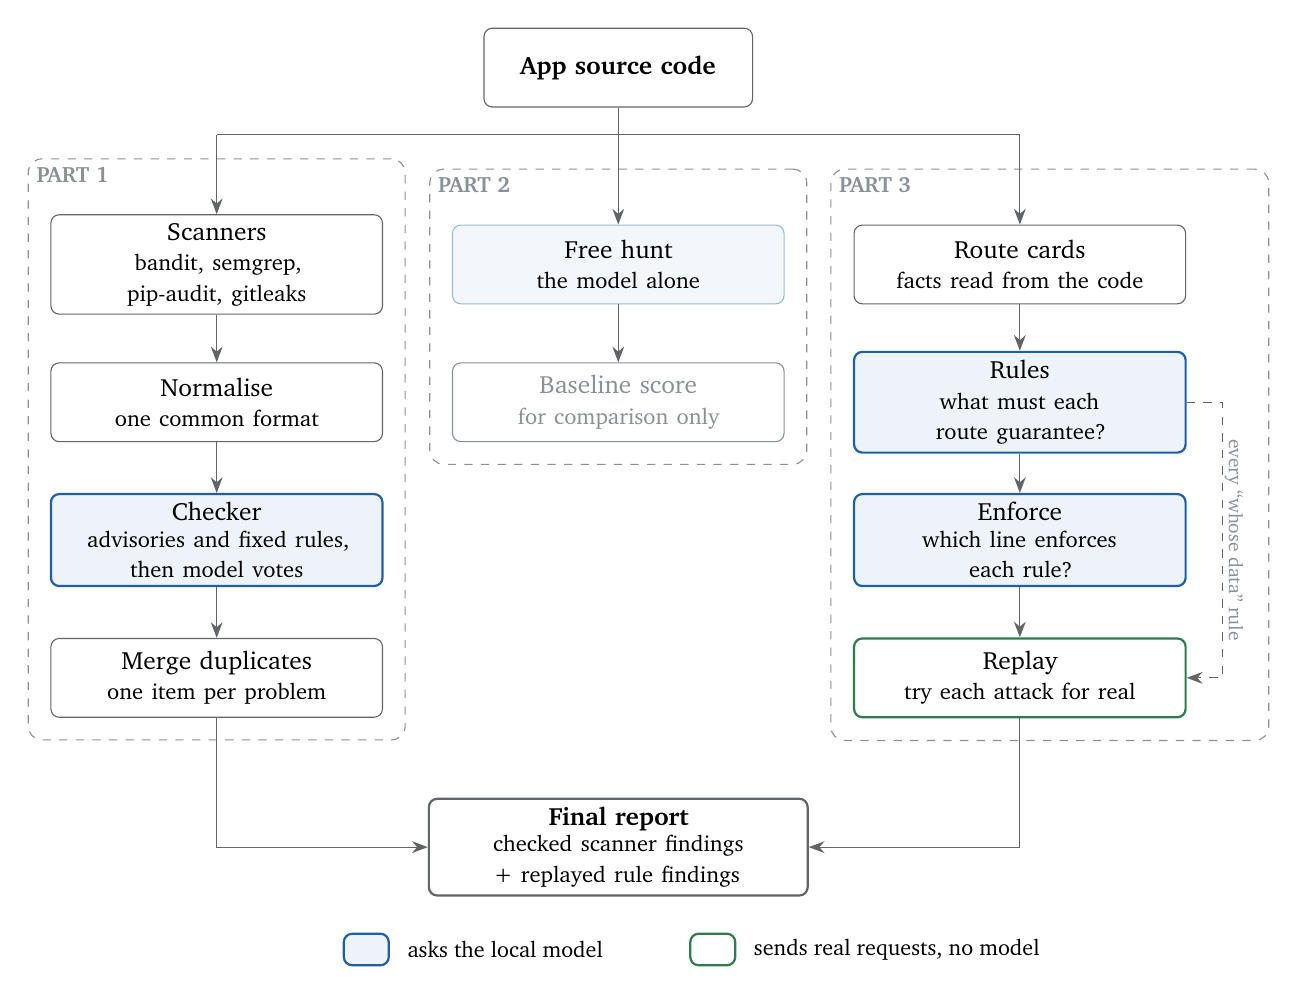
\begin{tikzpicture}[
  font=\small,
  box/.style={draw=ink!70,rounded corners=3pt,align=center,minimum height=10mm,text width=4.0cm,inner sep=3pt,fill=white},
  model/.style={box,draw=accent,fill=soft,thick},
  part/.style={draw=grey,dashed,rounded corners=5pt,inner xsep=8pt,inner ysep=8pt},
  arr/.style={-{Stealth[length=2mm]},draw=ink!70},
  lab/.style={font=\footnotesize\bfseries,text=grey,anchor=north west,inner sep=3pt}
]
\def\xa{-5.1} \def\xb{0} \def\xc{5.1}
\node[box,text width=3.2cm] (code) at (0,0) {\textbf{App source code}};
% Part 1
\node[box] (scan)  at (\xa,-2.5) {Scanners\\{\footnotesize bandit, semgrep, pip-audit, gitleaks}};
\node[box] (norm)  at (\xa,-4.25) {Normalise\\{\footnotesize one common format}};
\node[model] (check) at (\xa,-6.0) {Checker\\{\footnotesize advisories and fixed rules,\\ then model votes}};
\node[box] (merge) at (\xa,-7.75) {Merge duplicates\\{\footnotesize one item per problem}};
% Part 2
\node[model,draw=accent!45,fill=soft!70,thin] (hunt) at (\xb,-2.5) {Free hunt\\{\footnotesize the model alone}};
\node[box,draw=grey,text=grey] (base) at (\xb,-4.25) {Baseline score\\{\footnotesize for comparison only}};
% Part 3
\node[box] (card)  at (\xc,-2.5) {Route cards\\{\footnotesize facts read from the code}};
\node[model] (rules) at (\xc,-4.25) {Rules\\{\footnotesize what must each route guarantee?}};
\node[model] (enf)   at (\xc,-6.0) {Enforce\\{\footnotesize which line enforces\\ each rule?}};
\node[box,draw=good,thick] (rep) at (\xc,-7.75) {Replay\\{\footnotesize try each attack for real}};
% side path label (inside the Part 3 frame)
\node[font=\scriptsize,text=grey,rotate=-90,inner sep=1pt] (sidelab) at (7.82,-6.0) {every ``whose data'' rule};
% frames
\node[part,fit=(scan)(merge),yshift=6pt,inner ysep=14pt] (p1) {};
\node[lab] at (p1.north west) {PART 1};
\node[part,fit=(hunt)(base),yshift=6pt,inner ysep=14pt] (p2) {};
\node[lab] at (p2.north west) {PART 2};
\node[part,fit=(card)(rep)(sidelab),yshift=6pt,inner ysep=14pt] (p3) {};
\node[lab] at (p3.north west) {PART 3};
% output
\node[box,text width=4.6cm,thick] (out) at (0,-9.9) {\textbf{Final report}\\{\footnotesize checked scanner findings\\ + replayed rule findings}};
% arrows
\draw[draw=ink!70] (code.south) -- (0,-0.85);
\draw[draw=ink!70] (\xa,-0.85) -- (\xc,-0.85);
\draw[arr] (\xa,-0.85) -- (scan.north);
\draw[arr] (\xb,-0.85) -- (hunt.north);
\draw[arr] (\xc,-0.85) -- (card.north);
\draw[arr] (scan) -- (norm);  \draw[arr] (norm) -- (check);  \draw[arr] (check) -- (merge);
\draw[arr] (hunt) -- (base);
\draw[arr] (card) -- (rules); \draw[arr] (rules) -- (enf);   \draw[arr] (enf) -- (rep);
\draw[arr,dashed] (rules.east) -- ++(0.45,0) |- (rep.east);
\draw[arr] (merge.south) |- (out.west);
\draw[arr] (rep.south) |- (out.east);
% key
\node[model,minimum height=4mm,text width=5mm,inner sep=1pt] (k1) at (-3.2,-11.2) {};
\node[right=1mm of k1,font=\footnotesize] {asks the local model};
\node[box,draw=good,thick,minimum height=4mm,text width=5mm,inner sep=1pt] (k2) at (1.2,-11.2) {};
\node[right=1mm of k2,font=\footnotesize] {sends real requests, no model};
\end{tikzpicture}
\caption{The pipeline. Part~1: scanners plus a checker. Part~2: the model hunting alone, used only as a
yardstick. Part~3: route-by-route rule checking. Blue boxes ask the local model a question; every other box is
ordinary code. The dashed arrow: every ``whose data'' rule goes to replay, even one the enforce step accepted. The final report holds the scanner findings the checker kept and the rule findings replay confirmed or kept for a human to review.}
\label{fig:pipeline}
\end{figure}

\textbf{Why this order?} I wanted each part to earn its place with a number. Part~1 is the cheapest and
most reliable, so it came first. Part~2 told me exactly where the model fails on its own. Part~3 was
designed specifically for those failures.

\textbf{Who does what.} A recurring principle: the model is only used where judgement is genuinely needed,
and its answers are always checked by code. Anything code can decide on its own (Is this line really
there? Is this a dependency with a known advisory? Did the attack work?) is decided by code.

% ======================================================================
\section{What ``agent'' means here}
\label{sec:agent}

The brief left open what an agent is. I use the classic definition: an agent perceives its environment and
acts on it \cite{aima}. By this definition routeguard is an agent: it starts the app, logs in as different users,
sends attacks, observes what changed in the database and the response, and keeps or drops each claim based on what
it observed.

Giving the model control of the loop was not skipped; it was tried and measured. The free hunt in Part~2 had a
tool to ask for more code, and the model never used it (Section~\ref{sec:failed}). So the design puts the
\emph{control} in code and the \emph{judgement} in the model, and lets the environment (replay) have the last word.
What it is allowed to do follows from that: read the app's code, and send requests to an in-process copy of the
app as three test users. It has no network access and no tool that changes anything outside that copy.

\subsection{Agent mode: letting the model design the tests}
\label{sec:agentmode}

The free hunt gave the model control over \emph{what to read}. Agent mode (\code{agent/investigate.py}) tests the
other half: control over \emph{how each finding is tested}. For every rule the enforce step marks as broken, the model
designs the test: which user sends it, which field to change, which bad value to send, and which kind of probe to use.
The same code oracles as replay then decide whether the test proved anything, so the model never judges its own
test. For the dangerous probes (shell, file path, deserialisation, template) the model only names the kind and code
supplies the harmless payload, exactly as in replay. Both modes ran on vulny-app on the same 27 rules
(\code{tools/compare\_modes.py} lines them up rule by rule).

\begin{table}[H]
\centering
\caption{Replay vs agent mode on vulny-app, one run, hand-checked.}
\begin{tabularx}{\linewidth}{@{}Y c c c@{}}
\toprule
\textbf{Who designs the test} & \textbf{Bugs found} & \textbf{Confirmed by a real request} & \textbf{False confirmations} \\
\midrule
Code (replay) & 7/8 & 5 & 0 \\
The model (agent mode) & 4/8 & 4 & 0 \\
\bottomrule
\end{tabularx}
\end{table}

The agent confirmed nothing false: every test it ran either proved a real bug or proved nothing. Its failures were
quiet instead. For ``seats must not be negative'' it chose \code{:999999} as the bad value, which is not a number at
all, so the server never stored it and the negative-seats bug (V05) passed as safe. For the client-sent total (V04) and the role and credit
fields (V06) it chose a template-injection probe; that probe found nothing (or the request crashed), and the
agent counted the rule as safe, where replay keeps both for a human. So with a 7B model, \textbf{tests designed in code
stay the default}. The model's test design is worth using only where replay has no test at all, and then its
``safe'' verdicts should go to a human rather than remove the finding.

% ======================================================================
\section{Part 1: scanners plus a checker}

\subsection{Step 1: run four standard scanners}
Four free tools each read the code and report problems:

\begin{itemize}
  \item \textbf{bandit} and \textbf{semgrep} look for dangerous code patterns in Python and Flask.
  \item \textbf{pip-audit} checks whether the libraries the app uses have known security advisories.
  \item \textbf{gitleaks} looks for passwords and keys written into the code.
\end{itemize}

Each tool writes its results in its own format. \code{tools/normalize.py} converts all four into one list
with the same fields (tool, rule, file, line, quoted code, severity, CWE). It also hides any leaked secret,
so the report never repeats it. On cakeshop this gives \textbf{42 warnings}.

\subsection{Step 2: the checker decides which warnings are real}
Of those 42 warnings, only 31 point at real bugs (one bug often triggers several warnings), and 11 are false
alarms. The checker (\code{agent/verify.py}) sends each warning through the \emph{cheapest step that can
decide it}:

\begin{enumerate}
  \item \textbf{Dependency warning?} If pip-audit says a library version has a published advisory, it is real.
        No judgement needed.
  \item \textbf{Evidence check.} Is the code the scanner quoted really at that line (give or take 2 lines)?
        If not, the warning is rejected.
  \item \textbf{Group by line.} Several warnings on the same line are judged once.
  \item \textbf{Fixed rules, no model.} A handful of clear-cut cases: a warning on an \code{import} line is a
        false alarm; a secret read from the environment is fine, but a secret typed into the code is real;
        MD5 or SHA-1 used for passwords is real; \code{debug=True} is real; a database query built from text
        where every inserted name comes from a fixed allow-list is safe.
  \item \textbf{The local model}, for everything else. It sees the function around the flagged line, plus
        the context a human reviewer would look up: the decorators that protect the route, constants it uses,
        functions it calls, functions that call it, and for a web page the code that fills it.
\end{enumerate}

Two details make the model's judgement more trustworthy:

\begin{itemize}
  \item \textbf{It must reason before it decides.} The answer has to fill in, in this order: where the data
        comes from (\emph{source}), how it reaches the flagged line (\emph{path}), what protects it
        (\emph{protection}), and only then the \emph{verdict}. The scanner's own opinion is hidden so the model
        cannot simply agree with it.
  \item \textbf{It votes.} The same question is asked 3 times; the majority wins. If the vote is split, the
        question is asked again with twice as much context and 5 votes. If fewer than 4 of 5 agree, the warning
        is marked \emph{uncertain} and kept for a human to look at.
\end{itemize}


\subsection{Step 3: merge duplicates}
Scanners often report the same bug many times: bandit and semgrep on one line, or eight advisories for one
old library. \code{tools/merge\_findings.py} merges warnings that are on the same line, or in the same
function within 2 lines and either of the same weakness type or linked by a variable (one line builds a
value, the next line uses it). Each merged item keeps its original warnings, so nothing is lost.

\subsection{Results of Part 1 on cakeshop}

\begin{table}[H]
\centering
\caption{What the checker decided, per warning (42 warnings on cakeshop).}
\begin{tabular}{@{}l c c c l@{}}
\toprule
\textbf{Decided by} & \textbf{Warnings} & \textbf{Kept} & \textbf{Removed} & \textbf{Mistakes} \\
\midrule
Dependency advisory & 15 & 15 & 0 & none \\
Fixed rules & 10 & 4 & 6 & none \\
Local model & 17 & 15 & 2 & 3 false alarms kept \\
\midrule
\textbf{Total} & \textbf{42} & \textbf{34} & \textbf{8} & \\
\bottomrule
\end{tabular}
\end{table}

\begin{itemize}
  \item \textbf{No real bug was thrown away.} Removing false alarms is only useful if it never removes a
        real problem.
  \item 8 of 11 false alarms were removed: 6 by the fixed rules, only 2 by the model.
  \item After merging, the share of reported items that are real rose from \textbf{58\% to 79\%}, and the
        decoys flagged fell from \textbf{4 of 8 to 1 of 8}.
  \item The scanners hit \textbf{11 of 19} bugs. The checker cannot raise this number, because it only judges
        what the scanners report. Of the 8 missed, 6 are logic bugs that scanners cannot see by design.
\end{itemize}

\begin{lesson}
Most of the cleaning came from simple deterministic rules, not from the AI. The model was useful for the
cases in between, but it was the weakest judge in the chain.
\end{lesson}

% ======================================================================
\section{Part 2: what can the model do on its own?}
\label{sec:hunt}

Before building anything more complex, I measured the simplest possible approach: give the model the code
and ask it to find the bugs. This is the baseline every other part should beat. I tried three versions
(\code{agent/hunt.py}); all three ask the same open question (``find the security vulnerabilities'') with the
same list of things to look for, and differ only in what code the model sees:

\begin{itemize}
  \item \textbf{File by file.} The model reads each file whole and lists every vulnerability.
  \item \textbf{Route by route, as an ``agent''.} Inspired by the open-source tool Vulnhuntr \cite{vulnhuntr}. The model
        starts from each of the 21 routes and may ask to see the definitions of other functions (up to 4 per
        round, for up to 3 rounds) before it reports.
  \item \textbf{Route by route, with the full context} (\code{--mode context}, added later as a control). The
        model gets, for each route, exactly the code bundle Part~3 uses (Section~\ref{sec:prompts}): the route,
        its decorators, the functions it calls, constants, the before-request hook, the template and the table
        schema. It cannot ask for more, and needs not to: all 21 prompts fit the window with nothing left out.
\end{itemize}

The model had to copy the line it was reporting. That copy was used to fix line numbers (small models
miscount) and to catch invented code.

\begin{table}[H]
\centering
\caption{Free hunt vs.\ Part 1 on cakeshop (one run each). The context mode never sees \code{run.py},
\code{\_\_init\_\_.py} or \code{requirements.txt}, so the configuration and library bugs (V13, V14, V16--V18) are
out of its reach; compare it on the route bugs.}
\small
\begin{tabularx}{\linewidth}{@{}Y c c c c@{}}
\toprule
 & \textbf{Scanners + checker} & \textbf{Hunt: by file} & \textbf{Hunt: by route} & \textbf{Hunt: full context} \\
\midrule
Bugs hit (by location) & 11/19 & 9/19 & 7/19 & 10/19 \\
Bugs found \emph{for the right reason} (judged by hand) & 11 & 5 (+2 partly) & 1 (+2 partly) & 5 (+3 partly) \\
Logic bugs found for the right reason & 0/6 & 0/6 & 0/6 & 1/6 (+1 partly) \\
Findings that were a real bug & 79\% & 34\% & 31\% & 34\% \\
Decoys flagged & 1/8 & 2/8 & 4/8 & 5/8 \\
Time & -- & 9.4 min & 6.8 min & 8.9 min \\
\bottomrule
\end{tabularx}
\end{table}

\subsection{What went wrong}
\begin{itemize}
  \item \textbf{Zero of 6 logic bugs found for the right reason} in the first two versions. The model reacts to code that \emph{looks}
        dangerous; it does not reason about who is allowed to do what. A missing admin check was reported as
        ``SQL injection''; a negative order quantity as ``integer overflow''.
  \item \textbf{Three bad habits explain most false alarms.} Every database query was called SQL injection,
        even safe ones. Every \code{\{\{ \}\}} in a web page template was called cross-site scripting, even
        though the template engine escapes them. Form fields were called SQL injection.
  \item \textbf{It cannot tell decoys from bugs.} Its claim about a real path-traversal bug was word-for-word
        the same as its claim about a decoy protected by \code{secure\_filename}.
  \item \textbf{The ``agent'' never used its tool.} In 21 of 21 routes the model answered at once and never
        asked to see more code. So it missed a SQL injection whose dangerous part lived in another file.
\end{itemize}

\subsection{Is it the question or the context?}
The first two versions changed two things compared with Part~3: the question was open, and the model did not see
all the code. To separate the two, the third version gives the model Part~3's full context but keeps the open
question. The result splits cleanly:

\begin{itemize}
  \item \textbf{Context fixes the cross-file miss.} With \code{search\_products} from \code{db.py} in the prompt, the
        SQL injection that the agent version never asked for (V01) is found for the right reason.
  \item \textbf{Context barely helps with logic bugs.} 1 of 6 for the right reason (the IDOR on
        \code{/orders/<id>}: ``manipulate \code{order\_id} to access orders that do not belong to them''), and 1
        partly (the unprotected admin page, explained as ``the query does not filter by user\_id''). The negative
        quantity and the client-set price were both reported as ``a non-integer value raises \code{ValueError}'';
        making oneself admin and the missing CSRF protection were not reported at all.
  \item \textbf{More code means more false alarms.} 5 of 8 decoys were flagged, the most of any version: the
        allow-listed table and column names as SQL injection, the escaped search term as XSS, the
        \code{secure\_filename} route as path traversal. More lines in the prompt are more lines that look
        dangerous.
\end{itemize}

With the same context, the narrow questions of Part~3 wrote 8 of the 9 rules needed for these logic bugs
(Section~\ref{sec:rules}), and replay then confirmed them without accusing a single decoy. So the question explains
most of the gap, and the context a smaller part: it rescued one cross-file bug and one IDOR.

\subsection{What went right}
It found two bugs no scanner flagged: debug mode left on, and a path-traversal bug. So it is a useful
complement, not a replacement.

This matches published research: models asked to judge code directly perform close to chance on
realistic benchmarks and change their answers when variable names change \cite{primevul,steenhoek,secllmholmes}.


\begin{lesson}
This ``failed'' experiment set the direction for the rest of the project. The bugs everyone misses are
\emph{missing} lines. You cannot find a missing line by asking ``what looks dangerous?'', even with all the code
in front of you (the full-context control). You have to ask a different question.
\end{lesson}

% ======================================================================
\section{Part 3: checking each route against the rules it must follow}

\subsection{The idea}
Logic bugs are missing protections. So instead of asking the model to \emph{find} bugs, Part~3 turns the
problem around. For every route:

\begin{enumerate}
  \item \textbf{Write down what the route must guarantee.} Example: ``a user may only see their own order''.
  \item \textbf{Find the line that enforces each rule}, or say that none does.
  \item \textbf{For a rule nobody enforces, describe a request that breaks it.} Example: ``log in as Bob,
        open Alice's order''.
  \item \textbf{Check the claim with code}, and finally \textbf{send that request} to a local copy of the app
        and see what really happens.
\end{enumerate}

The model never searches for bugs. It answers small questions about 10 to 20 lines at a time, and code
checks every answer. This follows two published ideas: ABSENTIA \cite{absentia}, where splitting a web app
into routes and checking stated properties greatly improved finding broken access control, and Google
Project Zero's ``Naptime'' principle that a finding should be verified by a tool, not by the model's
opinion \cite{naptime}.

To stay general, the rules are never triggered by names (``a field called \code{quantity}'' or ``an address
starting with \code{/admin}''). That would only work on apps that happen to use those names. Instead, the
model gets a short list of rule \emph{types} taken from public security standards (OWASP Top 10, OWASP API
Security Top 10, OWASP ASVS \cite{owasptop10,owaspapi,owaspasvs}) and decides which apply.

\subsection{Step 1: route cards (no model)}
Before the model is asked anything, plain Python (\code{agent/routecard.py}) reads the code and builds a
\emph{route card} for every route. It holds only facts, no judgements:

\begin{itemize}
  \item what the route reads from the visitor (form fields, address parameters, cookies), including inside
        helper functions;
  \item which database tables it writes to, and their columns;
  \item which decorators protect it (such as \code{@login\_required}) and what checks those decorators do;
  \item which tables have an owner column such as \code{user\_id}.
\end{itemize}

A self-check confirms that every place the app reads visitor input appears on some card: on cakeshop,
0 are missing. The cards are not shown to the model; the later steps use them to decide what to ask, what
to check and what to send.

\subsection{Step 2: the rules each route must follow}
\label{sec:rules}
The model is asked what each route \emph{should} guarantee, not whether the code does it (that comes next).
After three rounds of experiments (Section~\ref{sec:failed}), the format that works best for a 7B model is
four short questions, each tied to an OWASP category:

\begin{enumerate}[label=\textbf{Q\arabic*},leftmargin=2.4em,itemsep=4pt]
  \item \textbf{Who may call this route?} The model picks one of: anyone, any logged-in user, admin.\\
        {\color{grey}Catches:} a missing login or admin check.
  \item \textbf{Whose record is it?} The model answers once per route.\\
        {\color{grey}Catches:} IDOR (one user reading or changing another user's record).
  \item \textbf{Does it change data?} Decided by \textbf{code}, not the model: a POST, a database write or a
        session change means the route needs CSRF protection.\\
        {\color{grey}Catches:} CSRF.
  \item \textbf{For \emph{each value} the visitor sends: what kind of value is it?} The model gives one answer per
        value: ordinary content, picks a record, the server must decide, needs limits, or the visitor must not set it.\\
        {\color{grey}Catches:} a client-set price, a negative quantity, a user making themselves admin.
\end{enumerate}

For Q4, each value is shown together with the lines of code where it ends up, for example:

\begin{lstlisting}
VALUE price: request.form['price'], converted with int()
   125 |     price = int(request.form["price"])
   126 |     total = price * quantity
   128 |     cur = db.execute(
   129 |         "INSERT INTO orders (user_id, product_id, quantity, total, ...
\end{lstlisting}

When a route loops over \emph{all} form fields and writes them to a table, each column of that table becomes
its own value. That is how \code{is\_admin} on the account page gets its own question.

\textbf{Result:} the model wrote 8 of the 9 rules needed to catch the labelled logic bugs, plus 92\% of the
rules I expected, with only 5 unnecessary rules out of 38. Compare that with \textbf{0 of 6} logic bugs found
by free hunting. The same model, asked a better question, does much better.

\subsection{Step 3: which line enforces each rule?}
For each rule, the model sees the rule and the code that runs for the route (the route, its decorators,
functions it calls, the page template, the table) and answers one of three things
(\code{agent/enforce.py}):

\begin{itemize}
  \item \textbf{enforced}: copy the line that enforces it;
  \item \textbf{not enforced}: copy the line where it breaks, and describe a request that breaks it;
  \item \textbf{not applicable}: the rule does not fit (Step 2 sometimes writes wrong rules).
\end{itemize}

Code then checks every ``enforced'' answer: the copied line must exist, and it must be part of the code that
actually runs for this route. If not, the answer becomes \emph{uncertain} and is kept as a finding.

\textbf{Example.} The page \code{/admin/orders} lists every customer's order, but nobody protects it.
Asked whether the rule ``only admins may call this'' is enforced, the model said \emph{yes}, and as proof
it quoted this line: \code{g.user['is\_admin']}. The code check noticed that this line lives inside a decorator
(\code{admin\_required}) that this route \emph{does not use}. The model's wrong ``yes'' was overruled, and the
bug stayed on the list.

Code does \emph{not} judge whether a quoted line really enforces the rule. That is the job of the next step.

\subsection{Step 4: replay the attacks (no model)}
This is the step that turns a claim into evidence. \code{agent/replay.py} takes each finding and sends a real
request to the app, using Flask's built-in test client and three test users: an admin, Alice and Bob. It keeps
only findings whose attack actually works.

There is one replay helper per rule \emph{type}, not one per bug, so nothing in it is specific to cakeshop:

\entryhead{Who may call}
\begin{fields}[2.9cm]
  \item[Request] A lower-level user opens the route: a normal user on an admin page, or a logged-out visitor on a
        login-only page.
  \item[Confirmed when] The page shows the victim's stored data.
\end{fields}
\entryhead{Whose data}
\begin{fields}[2.9cm]
  \item[Request] Bob opens or changes a record owned by Alice.
  \item[Confirmed when] Bob sees Alice's private data, or Alice's record is changed.
\end{fields}
\entryhead{Limits}
\begin{fields}[2.9cm]
  \item[Request] The value is sent out of range (for example $-5$).
  \item[Confirmed when] The server stores it.
\end{fields}
\entryhead{Must not change}
\begin{fields}[2.9cm]
  \item[Request] A normal user sends a field they must not set (\code{is\_admin=1}).
  \item[Confirmed when] That user's own account changes.
\end{fields}
\entryhead{Do not trust}
\begin{fields}[2.9cm]
  \item[Request] A harmless test payload chosen by where the value ends up: an outside address, \code{../} in a
        file name, \code{\{\{7*7\}\}}, a crafted cookie, or a shell character.
  \item[Confirmed when] The payload's own effect happens: an off-site redirect, source code returned, the number
        \code{49} on the page, or an empty marker file.
\end{fields}
\entryhead{CSRF}
\begin{fields}[2.9cm]
  \item[Request] The data-changing request without an anti-forgery token, as another website would send it.
  \item[Confirmed when] It still changes the database (or a cookie other than the session cookie).
\end{fields}

Replay logs in the way a browser does: it loads the login page, sends back its hidden fields (such as an
anti-forgery token) with the username and password, and stops with an error if a login is refused, rather than
silently testing as a logged-out visitor.

Everything specific to one app lives in a single small file, \code{replay\_config.json}: how to start the app,
where its database is, and which test users exist with which roles. A new app needs a new config file, not new
code. The payloads are deliberately harmless: the most a successful attack does is create one empty marker file
on my own machine.

\textbf{Result on cakeshop.} Step~3 produced 23 findings, of which 78\% pointed at real bugs. Replay kept 16,
and \textbf{all 16 pointed at a real bug} (94\% with the stricter scoring). It dropped 7 findings, for example:

\begin{itemize}
  \item ``login required'' on the cart pages, which are public by design and show no one's private data;
  \item an IDOR claim on the invoice page, where Bob actually gets ``not found'' for Alice's invoice. That
        page is a decoy that does check ownership, so replay correctly rejected a false accusation.
\end{itemize}

And it confirmed bugs by their real effect, not by the model's word: Bob makes himself an admin; Bob reads
Alice's order, message and note; a normal user reads the admin order list; a negative quantity is stored; a shell
character in an address parameter runs a command; \code{../} in an image name returns source code; a crafted
cookie runs code; a login link redirects to an outside site.

\begin{lesson}
Replay is what makes the rule step usable. The model's answers in Step~3 are noisy (on flask-webgoat, 17 rule
findings of which 10 were real), but a request either works or it does not. After replay, flask-webgoat was down
to 6 findings, all 6 real when checked by hand.
\end{lesson}

% ======================================================================
\section{How the model is prompted}
\label{sec:prompts}

The model is called in four places: the checker (Part~1), the free hunt (Part~2), and the rules and enforce steps
(Part~3). This section shows what each call sends, what it asks, what answer it expects, and what code does with
the answer. The prompts are in the source files (\code{SYSTEM\_PROMPT} in \code{verify.py}, \code{ROUTE\_SYSTEM} and
\code{VALUE\_SYSTEM} in \code{rules.py}, \code{SYSTEM} in \code{enforce.py}, three prompts in \code{hunt.py}); the
complete prompt and answer of every call is saved in the step's \code{*\_log.json}.

\subsection{What every call has in common}
\begin{itemize}
  \item \textbf{Structured output.} Every call goes to Ollama's \code{/api/chat} with a system message (the task) and a
        user message (the code). The request carries a JSON schema in Ollama's \code{format} field, so decoding is
        constrained: the answer is always valid JSON with the expected keys, and fields such as a verdict can only
        take values from a fixed list (an \code{enum}). No answer has to be parsed out of free text.
  \item \textbf{Reasoning before the verdict.} The model writes the keys in schema order, so the schema puts the
        reasoning fields first (\code{source}, \code{path}, \code{protection}, or \code{reason}) and the decision last.
        The verdict is then written \emph{after}, and conditioned on, the model's own account of the code. With the
        reason after the verdict, the reason only justified a decision already made (Section~\ref{sec:failed}).
  \item \textbf{Deterministic by default.} Single calls run at temperature 0 with a fixed seed, so a rerun gives the
        same answers. Votes use temperature 0.6 with seeds 0, 1, 2, so the three answers can differ. Repeat runs
        set \code{AGENT\_TEMP} and \code{AGENT\_SEED} (\code{agent/llm.py}).
  \item \textbf{A character budget.} The window (\code{num\_ctx}) is 2,048 or 4,096 tokens. The code budget is
        $(\text{num\_ctx} - \text{answer tokens}) \times 3.3$ characters minus the system prompt; code sections are
        dropped from the end until the prompt fits, and the prompt says how many were left out.
  \item \textbf{Code is shown as labelled, numbered sections.} Each section has a header with its role and file
        (\code{--- CALLED search\_products (cakeshop/db.py) ---}) and every line its number
        (\code{\ \ 111 | query = f"SELECT ..."}). In the checker the flagged line is marked \code{>>}.
  \item \textbf{Evidence is copied, then checked.} Whenever the model points at code it must copy the line, not only
        give a number. Code matches the copy against the file (ignoring quote style and whitespace) to fix wrong
        line numbers and to catch invented code.
  \item \textbf{What the model never sees:} the answer key, any comment hinting at a bug, and in the checker the
        scanner's own opinion (only the weakness type it suspects), so it cannot simply agree with it.
\end{itemize}

\subsection{The calls, one by one}

Each call below lists what the model is given, what it is asked, the answer it must return, and what code does
with that answer. ``Window'' is the context size (\code{num\_ctx}) and the maximum answer length, in tokens.

\entryhead{Checker \quad{\normalfont\small\color{grey}window 2,048 / 300, 3 votes}}
\begin{fields}
  \item[Input] The function around the flagged line (marked \code{>>}). As context only: the route's decorators,
        the constants it uses, the functions it calls, the functions that call it (one level up), and for a page,
        the view that fills it.
  \item[Question] Is the flagged line really exploitable, judging only protections visible in the code?
  \item[Answer] \code{source}, \code{path}, \code{protection}, then \code{verdict}: real, false\_positive or
        uncertain.
  \item[Code then] Takes the majority of 3 votes. A split vote is asked again with twice the window and 5 votes;
        if fewer than 4 of 5 agree, the warning is ``uncertain'' and kept for a human.
\end{fields}

\entryhead{Free hunt \quad{\normalfont\small\color{grey}window 4,096 / 900, 1 call}}
\begin{fields}
  \item[Input] A file (or a piece of one), or a route. Agent mode adds the definitions it asks for; context mode
        gives the full route bundle.
  \item[Question] Find the security vulnerabilities (with a list of kinds to look for).
  \item[Answer] A list of findings: \code{file}, \code{code}, \code{line}, \code{source}, \code{why},
        \code{title}, \code{cwe}, \code{severity}; agent mode also \code{need}.
  \item[Code then] Anchors the copied line in the file, removes duplicates, and scores against the answer key.
\end{fields}

\entryhead{Rules Q1 and Q2 \quad{\normalfont\small\color{grey}window 4,096 / 800, 1 call per route}}
\begin{fields}
  \item[Input] The route bundle: the route, its decorators (also a decorator that wraps another), constants,
        called functions, before-request hooks, templates and table schemas.
  \item[Question] What should this route guarantee: who may call it, and does it touch a record owned by one
        user? Judge from its purpose, not from its checks.
  \item[Answer] \code{who\_may\_call} (\code{reason}, then anyone, logged\_in\_user or admin) and
        \code{whose\_data} (\code{reason}, \code{applies}, \code{table}, \code{rule}).
  \item[Code then] Turns each answer into a rule for the enforce step (``only administrators may call
        /admin/orders'').
\end{fields}

\entryhead{Rules Q3 (CSRF) \quad{\normalfont\small\color{grey}no model}}
\begin{fields}
  \item[Code] Adds a CSRF rule when the route uses POST, PUT, PATCH or DELETE, writes to the database, or changes
        the session.
\end{fields}

\entryhead{Rules Q4 \quad{\normalfont\small\color{grey}window 4,096 / 800, 1 call per route}}
\begin{fields}
  \item[Input] The route code and every value the client sends, each with up to 8 lines where it is used.
  \item[Question] For each value: what kind of value is it?
  \item[Answer] Per value: \code{reason}, then \code{kind} (content, selects\_record, server\_decides,
        needs\_limits or must\_not\_set), then \code{rule}.
  \item[Code then] Turns server\_decides, needs\_limits and must\_not\_set into rules (do not trust, limits, must
        not change); the other two kinds need no rule.
\end{fields}

\entryhead{Enforce \quad{\normalfont\small\color{grey}window 4,096 / 600, 1 call per rule}}
\begin{fields}
  \item[Input] The route bundle, one rule, and for a value rule the lines where that value is used.
  \item[Question] Does the code enforce this rule?
  \item[Answer] \code{code}, \code{file}, \code{line}, \code{reason}, \code{status} (enforced, not\_enforced or
        not\_applicable), \code{attack}, \code{cwe}.
  \item[Code then] Accepts ``enforced'' only if the copied line exists and runs for this route (a quoted decorator
        must decorate it); otherwise the rule becomes ``uncertain''. Every unenforced or uncertain rule goes to
        replay.
\end{fields}

\subsection{Why the prompts are written this way}
\begin{itemize}
  \item \textbf{Counter the model's bias.} The checker's prompt opens with ``Automated flags are often false
        alarms'' and counts only protections ``VISIBLE in the code shown''. The first pushes against simply agreeing
        with the flag; the second stops the model from assuming a protection that exists somewhere it cannot see.
  \item \textbf{Separate ``should'' from ``does''.} The rules prompts say: \emph{judge from what the route is FOR: its
        URL, the data it reads or writes, the page it shows. Do not base your answer on decorators or checks in the
        code; whether they are right is tested later.} The intent: a rule derived from the existing checks would only
        restate what the code already does, so a missing check could never show up. The second question (does the code
        do it?) is a separate call, enforce.
  \item \textbf{Closed choices, not free lists.} Round~1 asked for a free list of rules and got filler; round~2 asked
        yes/no per rule type and almost never produced value rules. Round~3 asks one closed question per value, with
        the five kinds defined in one line each, which is what a small model answers reliably
        (Section~\ref{sec:failed}).
  \item \textbf{Show where a value goes.} Q4 shows each value next to the lines that use it, because the kind of a
        value depends on where it ends up (a price that becomes an order total, an \code{is\_admin} column that a loop
        writes).
  \item \textbf{Make claims testable.} Enforce must copy the enforcing line, and for a broken rule describe one
        request (``who is logged in, method, URL, values, what happens''). The copy is what code checks; the request
        is what replay turns into a real one.
\end{itemize}

\subsection{An example, end to end}
For \code{GET /orders/<id>} the rules step answered \code{whose\_data} with: ``Only the user whose `id' matches the
`user\_id' in the `orders' table should be able to access this route.'' Enforce was then sent the route bundle and
that rule, and answered:

\begin{lstlisting}
{"code": "@login_required", "file": "cakeshop/auth.py", "line": 14,
 "reason": "The @login_required decorator checks if a user is logged in, but it
            does not verify that the logged-in user is the owner of the order.",
 "status": "not_enforced",
 "attack": "A user who is logged in as another user can access the order detail
            of that other user by visiting /orders/<order_id> ...",
 "cwe": "CWE-284: Improper Access Control"}
\end{lstlisting}

Code turned this into a finding on the route (CWE-639, the type fixed for ``whose data'' rules, not the model's
label), and replay logged in as Bob and opened Alice's order: the page showed her private cake message, so the
finding was confirmed. The same route in Q4 also shows a typical error: for \code{POST /checkout}, the model
classed \code{price} as \code{needs\_limits} (``price must be a positive integer'') instead of
\code{server\_decides}, which is why the client-set price (V05) is reported with the wrong explanation
(Section~\ref{sec:misses}).

% ======================================================================
\section{How the agent explains a result}
\label{sec:explain}

A finding is only useful if a developer can act on it. The last step, \code{tools/report.py}, turns the saved
outputs into one readable report per app (\code{runs/report.md}). It adds no new judgement; it shows, for each
problem, where it is (file, line, route and a code excerpt), what is wrong in plain words, why the agent believes it
(which scanner flagged it and the checker's source, path and protection, or the rule the route breaks and the model's
reading of the code), the evidence (the request replay sent, as which user, and what changed), and how to fix it.
Findings that point at the same problem are shown once, and each is marked \emph{confirmed by a real request},
\emph{judged real by the checker (not tested)} or \emph{needs human review}. A last section lists the suspicions replay tested
and cleared, and what the report does not cover. One entry, shortened:

\begin{lstlisting}
### 4. Missing authorisation on GET /admin/orders
Confirmed by a real request . severity estimate: high . CWE-862
Where: cakeshop/admin.py:12
What is wrong: The route does not check that the caller has the role it needs.
Why the agent reports it:
- Rule this route must follow: Only administrators may call /admin/orders.
- Which line enforces it? The model's answer failed the code check (the copied
  line is not in the code), so the rule is treated as not enforced.
- Replay: As bob (a normal user): GET /admin/orders -> 200.
- Outcome: bob received alice's data 'Chilonzor 12, Tashkent' -- no access check.
How to fix: Protect the route with the role check the app already uses
(e.g. @admin_required) and test it with a normal account.
\end{lstlisting}

The severity shown is an estimate from the type of weakness alone, and the report says so. When the model's
weakness label for an untested finding may be wrong (it once called a client-sent total ``command injection''), the
report describes the finding by the rule it breaks instead.

% ======================================================================
\section{Measuring fairly}

A result is only as honest as the way it is scored. \code{tools/score.py} compares any list of findings with the
answer key.

\begin{itemize}
  \item \textbf{Normal scoring} counts a bug as found if a finding points within 2 lines of it.
  \item \textbf{Strict scoring} (\code{--strict}) also requires the right weakness type (CWE). Without it, an IDOR
        bug can be ``found'' by a finding that wrongly calls it SQL injection. Strict scoring is a lower bound: it
        misses right answers labelled with a neighbouring CWE number.
  \item For the free-hunt baseline, I also \textbf{judged every finding by hand}, because the two automatic scores
        disagree there.
  \item \textbf{The results in this report are checked by hand.} The automatic score is a quick first pass: a
        finding that reports the right bug but points at a nearby line (for example the route's first line)
        falls outside its 2-line window, and a real problem the answer key forgot counts as wrong. So every
        finding it did not credit was checked against the code and the replay log. Each decision, with its
        reason, is written in \code{labels/hand\_check.json}, and \code{score.py --hand} applies it, so the hand
        numbers can be reproduced and challenged.
\end{itemize}

I also fixed two problems in my own scoring. The first version said 24 of 64 copied lines were ``invented''
by the model. Checking by hand, most were real lines with \code{'} instead of \code{"}, or a multi-line statement
written on one line. The matcher now ignores such differences, and only 2 of 64 are truly invented. Second, I
report precision per \emph{merged item}, not per warning: per warning it looked better (91\%) only because
duplicate dependency warnings are always right.

% ======================================================================
\section{Results}
\label{sec:results}

The ``full system'' is the output of Part~1 (scanners + checker) together with the confirmed findings from Part~3
(replay).

\begin{figure}[H]
\centering
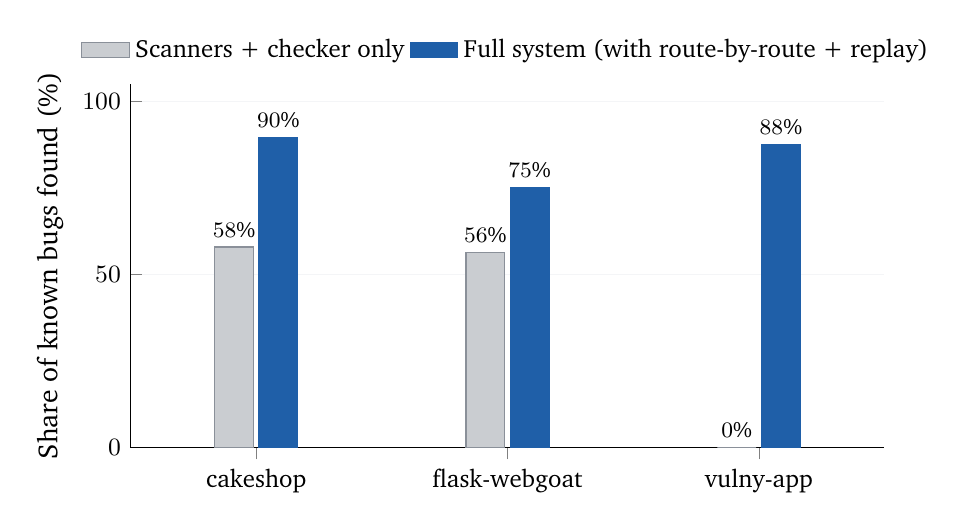
\begin{tikzpicture}
\begin{axis}[
  ybar, bar width=14pt, area legend, width=0.92\linewidth, height=6.2cm,
  ymin=0, ymax=105, ylabel={Share of known bugs found (\%)},
  symbolic x coords={cakeshop,flask-webgoat,vulny-app},
  xtick=data, enlarge x limits=0.25,
  legend style={at={(0.5,1.03)},anchor=south,legend columns=2,draw=none,font=\small},
  nodes near coords={\pgfmathprintnumber[fixed,precision=0]{\pgfplotspointmeta}\%},
  nodes near coords style={font=\footnotesize},
  axis lines*=left, ymajorgrids, grid style={draw=lightgrey},
  tick label style={font=\small}
]
\addplot[fill=grey!45,draw=grey] coordinates {(cakeshop,57.9) (flask-webgoat,56.25) (vulny-app,0)};
\addplot[fill=accent,draw=accent] coordinates {(cakeshop,89.5) (flask-webgoat,75) (vulny-app,87.5)};
\legend{Scanners + checker only, Full system (with route-by-route + replay)}
\end{axis}
\end{tikzpicture}
\caption{Recall on each app, checked by hand. cakeshop: 11/19 $\to$ 17/19. flask-webgoat: 9/16 $\to$ 12/16
(automatic score 11/16). vulny-app: 0/8 $\to$ 7/8 (automatic score 6/8). One run each.}
\label{fig:recall}
\end{figure}

\begin{table}[H]
\centering
\caption{Full results, checked by hand: bugs found, and the share of reported findings that are real
security problems (library advisories for the pinned versions count as real). In brackets, the automatic score
(\code{tools/score.py} without \code{--hand}), which only credits findings within 2 lines of the answer key's mark
and counts problems the answer key does not list as wrong.}
\small
\begin{tabularx}{\linewidth}{@{}Y *{5}{>{\centering\arraybackslash}p{2.15cm}}@{}}
\toprule
\textbf{App} & \textbf{Bugs / decoys} & \textbf{Scanners + checker} & \textbf{Replay only} & \textbf{Full system: found (automatic)} & \textbf{Full system: precision (automatic)} \\
\midrule
cakeshop & 19 / 8 & 11/19, 79\% & 9/19, 100\% & 17/19 (17/19) & 90\% (90\%) \\
flask-webgoat & 16 / 0 & 9/16, 91\% & 6/16, 100\% & 12/16 (11/16) & 94\% (76\%) \\
vulny-app & 8 / 5 & 0/8, 75\% & 7/8, 64\% & 7/8 (6/8) & 67\% (33\%) \\
\bottomrule
\end{tabularx}
\end{table}

\subsection{How to read these numbers}
\begin{itemize}
  \item \textbf{On cakeshop}, the route-by-route part adds exactly the bugs that scanners cannot see: IDOR,
        self-promotion to admin, the missing admin check, negative quantities and CSRF, each confirmed by a real
        request. Only 1 of 8 decoys was flagged.
  \item \textbf{On flask-webgoat}, most bugs are code-pattern or configuration bugs, so Part~1 does most of the
        work. Part~3 adds CSRF, and confirms the command injection by actually running a command.
  \item \textbf{On flask-webgoat}, all 6 replayed findings point at real bugs (the automatic score credits only 4,
        because two sit more than 2 lines from where the answer key anchors the bug). Only 2 of the 6 were
        confirmed by an effect; the other 4 are kept as
        ``uncertain'' because replay has no test payload for that kind of weakness yet.
  \item \textbf{On vulny-app}, the scanners find nothing, as expected for an app with only logic bugs, so everything
        comes from Part~3. It is analysed bug by bug in the next section.
\end{itemize}

\subsection{Testing Part 3 on logic bugs it has never seen}
\label{sec:vulny}

On vulny-app, Part~3 put 7 of the 8 bugs on its list (the automatic score says 6; one finding sits 3 lines from
the line the answer key marks), confirmed 5 of them with a real request, and flagged none of the 5 decoys,
including the ones protected by a helper in another file and by a decorator wrapping another decorator.


Bug by bug:

\begin{itemize}[itemsep=3pt]
  \item \textbf{V01 Workshop management page open to any member.} \st{warn}{Missed.} The rules step decided that
        any logged-in user may open \code{/workshops/manage}, so the missing staff check was never questioned.
  \item \textbf{V02 Booking receipt open without logging in.} \st{good}{Confirmed.} A logged-out visitor received
        Alice's receipt; Bob could read it too.
  \item \textbf{V03 Any member can view another member's booking.} \st{good}{Confirmed.} Bob opened Alice's booking.
  \item \textbf{V04 Booking total taken from the form.} \st{accent}{Found, kept as uncertain.} The rules step said
        the server must decide the total, but replay has no test for this kind of value yet. The model labelled it
        with the wrong weakness type, so strict scoring does not count it.
  \item \textbf{V05 Seat count accepts zero or negative values.} \st{good}{Confirmed.} The server stored a booking
        for $-5$ seats.
  \item \textbf{V06 Profile update writes role and credit from the form.} \st{accent}{Found, kept as uncertain,} for
        the same reason as V04.
  \item \textbf{V07 Profile form has no CSRF protection.} \st{good}{Confirmed.} A forged request without the token
        changed the database.
  \item \textbf{V08 Any member can cancel another member's booking.} \st{good}{Confirmed.} Bob's request changed
        the status of Alice's booking. The scorer misses it only because the finding is 3 lines from the label.
\end{itemize}

\begin{itemize}
  \item \textbf{Every confirmed finding was real.} Replay kept 15 findings: 7 confirmed, all real (the 5 bugs above,
        a second finding on V02, and one bug the answer key does not list, below), and 8 uncertain
        (left for a human), of which 3 are real (V04 and the two fields of V06) and 5 are noise (range warnings on
        staff and admin forms, and CSRF on logout).
  \item \textbf{The answer key missed two real bugs.} The booking-cancel and seat-booking forms have no CSRF check
        either. The first was confirmed by replay; the second was missed, because the enforce step accepted a line
        in the before-request hook (the one that creates the token) as the route's protection.
  \item \textbf{Full-system precision is 67\%.} Of the 18 findings, 12 point at a real problem: 9 in the app
        and 3 security advisories for the pinned Flask, Werkzeug and click versions. The other 6 are the noise above
        and one scanner warning about converting a form value to a number. (The automatic score says 33\%: it
        counts the advisories and the unlisted CSRF bug as wrong, and misses V08 by 3 lines.)
  \item The model steps (route cards, rules, enforce) ran once on this app, with no change to any prompt or rule.
\end{itemize}

\subsection{Every missed bug: looked at, or never looked for?}
\label{sec:misses}

For each bug the automatic score marks as missed, I went back to the logs of every step (scanner warnings, the
checker's verdicts, the rules, the enforce answers and the replay requests) to see whether the system had looked at
the bug and got it wrong, or had never looked for it at all. The automatic score, counted strictly, marks 11 bugs as
missed. Four of them were in fact found (group B) and are counted as found in the headline results, so 7 bugs were
really missed:

\begin{itemize}[itemsep=3pt]
  \item \textbf{A. Looked at, wrong answer (2 bugs).} The bug was in front of the system, and it answered wrongly.
  \item \textbf{B. Found; only the automatic score misses it (4 bugs).} The system reported the right bug, but a
        few lines away from the marked line or with a neighbouring weakness label. These are counted as found.
  \item \textbf{C. Outside what the system looks at (5 bugs).} No scanner rule, no route and no rule type covers
        it, so the code was never examined.
\end{itemize}

\entryhead{cakeshop: 2 bugs missed}
\begin{itemize}[itemsep=3pt]
  \item \textbf{V05 Client-controlled price at checkout.} \grp{A}\\
        The rules step did ask about \code{price} on \code{/checkout}, but answered ``needs limits'' (``price must
        be a positive integer'') instead of ``the server must decide''. A price of 1 would pass that rule. Replay
        then sent \code{price=-5} and the server stored it, which does prove that the client sets the price, but
        the finding carries the ``limits'' weakness type, so the scorer files it under the negative-quantity bug
        (V06).
  \item \textbf{V14 Flask debug mode.} \grp{C}\\
        The checker has a fixed rule for \code{debug=True}, but it only judges lines that a scanner flagged, and no
        scanner flagged cakeshop's \code{run.py} (bandit's debug rule did fire on flask-webgoat). Route checking
        only looks at routes, and \code{app.run()} is not one. The free-hunt baseline found it, but the free hunt
        is not part of the full system.
\end{itemize}

\entryhead{flask-webgoat: 6 bugs missed with strict scoring (5 with normal scoring)}
\begin{itemize}[itemsep=3pt]
  \item \textbf{V05 Path traversal when writing a message file.} \grp{B}\\
        Found. The rules step wrote ``the filename must be sanitised'', enforce said no line does it, and replay
        kept the finding as ``uncertain'' because it has no test payload for file writes. The finding is labelled
        as command injection (CWE-78), so normal scoring counts it and strict scoring does not.
  \item \textbf{V06 Open redirect after a failed login.} \grp{B}\\
        Found. The rules step wrote ``the URL must be validated'' and replay kept it as ``uncertain'': the redirect
        only happens after a \emph{failed} login, which the replay helper does not try. The finding points at the
        line that reads \code{url}, more than 2 lines from where the answer key anchors the bug, so the scorer does
        not match them.
  \item \textbf{V07 Every SQL statement, passwords included, printed to the log.} \grp{C}\\
        Never examined. The logging is switched on once, in the database setup, not in a route:
        \code{set\_trace\_callback(print)}. No scanner has a rule for it and no rule type asks about logging.
  \item \textbf{V08 CORS allows any origin.} \grp{C}\\
        Never examined. The header is set in an \emph{after}-request hook in \code{run.py}. Route cards collect
        only \emph{before}-request hooks, so this code is on no card. No scanner rule and no rule type covers
        response headers.
  \item \textbf{V09 Content Security Policy allows inline scripts.} \grp{C}\\
        Same as V08: set in the same after-request hook, out of view.
  \item \textbf{V12 Passwords stored in plain text.} \grp{C}\\
        Never looked for. The checker can confirm weak hashing (MD5, SHA-1) when a scanner flags it, but a password
        that is not hashed at all leaves no dangerous line to flag, and no rule type asks how passwords are stored.
\end{itemize}

\entryhead{vulny-app: 3 bugs missed with strict scoring (2 with normal scoring)}
\begin{itemize}[itemsep=3pt]
  \item \textbf{V01 Workshop management page open to any member.} \grp{A}\\
        The rules step did ask who may open \code{/workshops/manage}, but answered ``any logged-in user'' instead of
        ``staff''. With that rule, the route's login check counts as enough, and the missing staff check is never
        questioned.
  \item \textbf{V04 Booking total taken from the form.} \grp{B}\\
        Found. The rules step answered ``the server must decide'' for \code{total\_cost}, and replay kept the
        finding as uncertain. The model labelled it as command injection (CWE-78), so strict scoring does not
        count it.
  \item \textbf{V08 Any member can cancel another member's booking.} \grp{B}\\
        Found and confirmed by replay (Bob's request changed Alice's booking), but the finding points 3 lines above
        the line the answer key marks, so the scorer does not match them.
\end{itemize}

\begin{lesson}
Only two misses are plain wrong answers from the model, both in the rules step: a value judged as ``needs
limits'' instead of ``the server must decide'' (cakeshop V05), and a staff page judged open to any member
(vulny-app V01). Four more are not misses at all: the system found them, and only the automatic score does not
accept them. The other five sit \emph{outside} what the
system examines: start-up settings, code that runs after a request, response headers, logging, and how passwords
are stored. The route-by-route design sees routes well and little else, which tells me exactly where to extend it
next.
\end{lesson}

% ======================================================================
\section{Experiments that failed, and what they taught}
\label{sec:failed}

Several experiments did not work. These are the ones that changed the design.

\entryhead{Rule-based discovery of logic bugs (an early version)}
\begin{fields}[3cm]
  \item[What happened] It worked on cakeshop, but it triggered on names such as \code{quantity} or \code{/admin},
        so it would not carry over to other apps.
  \item[What I changed] Deleted it. Replaced by rule \emph{types} from OWASP that the model applies to each route.
\end{fields}
\entryhead{Security notes per weakness type (12 notes from OWASP and the Flask docs in the checker's prompt)}
\begin{fields}[3cm]
  \item[What happened] Identical score with and without them. One verdict improved, one got worse. A decoy stayed
        a false alarm even though its note explained exactly why it is safe.
  \item[What I changed] Removed them: no evidence they help.
\end{fields}
\entryhead{Letting the model write a ``reason'' after its verdict}
\begin{fields}[3cm]
  \item[What happened] The reason was written \emph{after} the decision, so it justified the decision rather than
        informing it.
  \item[What I changed] The reasoning fields now come \emph{before} the verdict.
\end{fields}
\entryhead{Free hunt with a tool loop (Vulnhuntr style)}
\begin{fields}[3cm]
  \item[What happened] The model never asked for more code, in 21 of 21 routes.
  \item[What I changed] Kept it as a baseline; Part~3 gives the model the code it needs up front.
\end{fields}
\entryhead{Agent mode: the model designs each replay test (Section~\ref{sec:agentmode})}
\begin{fields}[3cm]
  \item[What happened] On vulny-app it found 4 of 8 bugs instead of 7, with no false confirmation, but three real
        bugs passed as safe after a badly chosen value or probe.
  \item[What I changed] Kept as an experiment; the tests stay designed in code.
\end{fields}
\entryhead{Rules, round 1: a free list of 6 rule types}
\begin{fields}[3cm]
  \item[What happened] The model filled in every type; 30 of 35 extra rules were filler such as ``this route does
        not need CSRF protection''.
  \item[What I changed] Moved to round 2.
\end{fields}
\entryhead{Rules, round 2: a yes/no checklist}
\begin{fields}[3cm]
  \item[What happened] The filler was gone and CSRF was right, but value rules were almost never written, and the
        login redirect bug was missed in all 5 runs of rounds 1 and 2.
  \item[What I changed] Round 3: one answer per value, which found the redirect for the first time.
\end{fields}
\entryhead{Accepting the model's ``yes, it is enforced''}
\begin{fields}[3cm]
  \item[What happened] On the order page the model wrongly said that ownership was checked.
  \item[What I changed] Replay now tests every ``whose data'' rule, including the ones the model accepted.
\end{fields}

\begin{lesson}
Two general points. First, \textbf{the format of the question mattered more than the information given}: free list,
then checklist, then one answer per value. Second, \textbf{I stopped tuning on purpose}. Every fix found by looking
at cakeshop's answer key makes cakeshop's numbers less trustworthy. On the outside apps, no prompt or rule was
changed after seeing their results.
\end{lesson}

% ======================================================================
\section{Limitations}
\label{sec:limits}

\begin{itemize}
  \item \textbf{Small sample.} Three small, deliberately vulnerable apps. A real business codebase, where most code
        is fine, would stress false alarms far more.
  \item \textbf{Single runs.} Every number comes from one run. The model's answers can change between runs. The
        pipeline already supports repeat runs (\code{AGENT\_TEMP}, \code{AGENT\_SEED}), but I have not run them yet.
  \item \textbf{Answer keys.} cakeshop's key and prompts were developed together. flask-webgoat's key was fixed
        before its run; vulny-app's was written by the model that generated the app and read only after the run.
  \item \textbf{vulny-app is generated.} Its bugs are textbook examples planted on request, so it is easier than real
        code, and its own answer key missed two real bugs.
  \item \textbf{Hand checking.} The final counts were checked by hand by me, against the code and the replay logs.
        Every decision is written down in \code{labels/hand\_check.json}, but a second person checking them would
        make them stronger.
  \item \textbf{Scoring by location} can credit a finding with the wrong explanation; strict scoring can miss a right
        finding with a neighbouring CWE number.
  \item \textbf{Python/Flask only.} Route cards do not yet understand database ORMs (SQLAlchemy models), class-based
        views or some ways of registering routes.
  \item \textbf{Checker context.} When a function has many callers, the last ones may be cut to fit the model's short
        window, and the dangerous caller may be among them. Callers are followed only one level up.
  \item \textbf{Merging is a guess} from location and data flow; two different bugs on nearby lines could be merged.
  \item \textbf{Replay needs each app's own libraries}, and the test apps pin incompatible versions. flask-webgoat was
        replayed with a newer Flask than it pins; the replayed bugs do not depend on the version, but the environment
        did not match exactly.
\end{itemize}

% ======================================================================
\section{Next steps}

\begin{enumerate}
  \item \textbf{Identity and session rules.} Follow the code \emph{inside} before-request hooks (today only the
        hook's own lines are shown), and add a rule type for ``can a user forge who they are?'' (for example a
        login cookie that is not signed), with a replay that edits the attacker's own cookie to name the victim.
  \item \textbf{A stricter enforce check.} A line in a before-request hook runs for every route, so it should not
        count as one route's protection unless it really checks something; on vulny-app this let a missing CSRF check
        through.
  \item \textbf{Look beyond routes.} Collect after-request hooks (response headers such as CORS and CSP) and
        app start-up code (debug mode, logging), and add a check for how passwords are stored.
  \item \textbf{Output escaping.} A rule for values that reach a page through \code{|safe} or \code{Markup}.
  \item \textbf{Replay tests for the remaining value kinds}, such as a total or a role sent by the client, which are
        found today but only kept as uncertain.
  \item \textbf{More replay payloads}, so findings now kept as ``uncertain'' can be confirmed or dropped.
  \item \textbf{Bounded autonomy, where code has no test.} Agent mode (Section~\ref{sec:agentmode}) showed the
        model's tests lose bugs that code-designed tests catch. Use it only for findings replay cannot test yet,
        and send its ``safe'' verdicts to a human instead of dropping the finding.
  \item \textbf{Repeat runs}, to measure how stable each number is.
  \item \textbf{A real, non-deliberately-vulnerable codebase}, where false alarms matter more than recall.
\end{enumerate}

% ======================================================================
\section{How to run it, and safety}

\subsection{Requirements}
You need four things: the scanners (listed in \code{requirements-agent.txt}); gitleaks; Ollama with the
\code{qwen2.5-coder:7b} model; and a separate Python environment with the target app's own libraries (for replay). The agent code itself uses only the
Python standard library.

\begin{lstlisting}[language=bash]
python3 -m venv agentenv && agentenv/bin/pip install -r requirements-agent.txt
python3 -m venv appenv && appenv/bin/pip install -r cakeshop/requirements.txt
ollama pull qwen2.5-coder:7b
./run.sh cakeshop
scripts/get_test_apps.sh      # only for flask-webgoat
\end{lstlisting}

\code{run.sh} runs every step in order: scanners, normalising, checker, merging, route cards, rules, enforce,
replay, the readable report (\code{runs/report.md}), and finally scoring if an answer key is present. Each step can also be run on its own and reads and writes
fixed files, so any intermediate result can be inspected. \code{rerun.sh} re-runs everything after the scanners and
saves the outputs under \code{runs/<tag>/}.

\subsection{Safety boundaries}
\begin{itemize}
  \item The agent was only ever run on code I wrote (cakeshop) or on public, deliberately vulnerable training apps.
  \item Replay attacks a copy of the app inside the test process, bound to \code{127.0.0.1}. No third-party system is
        scanned or contacted.
  \item Attack payloads are harmless by design: the strongest one creates a single empty marker file.
  \item Leaked secrets found by gitleaks are masked in the agent's output.
  \item The model runs locally; no code leaves the machine.
\end{itemize}

% ======================================================================
\section{Conclusion}

The question behind this project was how to make an AI system reason like a useful security-focused coding agent. On a small local model,
my answer is to \textbf{change the job the model is given}. Asked to ``find vulnerabilities'', it guessed from
appearances and found at most one of the six logic bugs for the right reason, even with all the route's code
in front of it. Asked smaller questions (what must this route
guarantee, which line enforces it), with code checking each answer and real requests confirming each attack, the same
7B model helped the system go from 11 to 17 of 19 bugs on my test app while keeping 90\% of its findings real.
On vulny-app, an app built around exactly these logic bugs that I had never seen, it found 7 of 8, confirmed 5 of
them with a real request, every confirmed finding was real, and none of the 5 decoys was flagged.

The most valuable parts turned out not to be the AI at all: the deterministic rules in the checker, the fact-only route
cards, and the replay step that tries every attack. The model is one useful component among them, used only where
judgement is needed, and never trusted on its own word.

% ======================================================================
\appendix
\section{The planted bugs and decoys}
\label{app:bugs}

\subsection{cakeshop}

\begin{table}[H]
\centering
\small
\caption{The 19 planted vulnerabilities.}
\begin{tabular}{@{}l l l l@{}}
\toprule
\textbf{ID} & \textbf{Vulnerability} & \textbf{Type} & \textbf{CWE} \\
\midrule
V01 & SQL injection in product search (across two files) & pattern & 89 \\
V02 & Server-side template injection in cake-message preview & pattern & 1336 \\
V03 & Path traversal in cake image endpoint & pattern & 22 \\
V04 & Insecure deserialisation of the cart cookie (pickle) & pattern & 502 \\
V05 & Client-controlled price at checkout & logic & 602 \\
V06 & Unvalidated quantity allows zero or negative orders & logic & 1284 \\
V07 & Stored XSS in product reviews & pattern & 79 \\
V08 & IDOR: any logged-in user can view any order & logic & 639 \\
V09 & OS command injection in invoice generation & pattern & 78 \\
V10 & Missing authorisation on admin order list & logic & 862 \\
V11 & Mass assignment lets users make themselves admin & logic & 915 \\
V12 & Open redirect after login & pattern & 601 \\
V13 & Hard-coded, guessable session secret key & config & 798 \\
V14 & Flask debug mode enabled & config & 489 \\
V15 & Passwords hashed with unsalted MD5 & pattern & 916 \\
V16--V18 & Vulnerable Flask, Werkzeug and Jinja2 versions & dependency & 1395 \\
V19 & No CSRF protection on any state-changing form & logic & 352 \\
\bottomrule
\end{tabular}
\end{table}

\begin{table}[H]
\centering
\small
\caption{The 8 decoys: code that looks dangerous but is safe.}
\begin{tabularx}{\linewidth}{@{}l >{\raggedright\arraybackslash}p{5.2cm} Y@{}}
\toprule
\textbf{ID} & \textbf{Looks like} & \textbf{Why it is safe} \\
\midrule
D01 & Text-built SQL with a table name & The table name must be in a fixed allow-list \\
D02 & Running a system command & Fixed argument list, no shell, no visitor input \\
D03 & Building a template from a string & Visitor input is passed as an escaped variable, not pasted into the template \\
D04 & Serving a file by name & \code{secure\_filename} and \code{send\_from\_directory} block \code{../} \\
D05 & An admin page & Protected by \code{@admin\_required}, defined in another file \\
D06 & Text-built SQL UPDATE with column names & Column names checked against a list; values passed safely \\
D07 & Invoice lookup by ID & The query is restricted to the current user's orders \\
D08 & Search term shown back on the page & The template engine escapes it automatically \\
\bottomrule
\end{tabularx}
\end{table}

\subsection{vulny-app}
\label{app:vulny}

\begin{table}[H]
\centering
\small
\caption{The 8 planted vulnerabilities in vulny-app (all logic bugs).}
\begin{tabular}{@{}l l l@{}}
\toprule
\textbf{ID} & \textbf{Vulnerability} & \textbf{CWE} \\
\midrule
V01 & Workshop management page accessible to any member & 862 \\
V02 & Booking receipt accessible without logging in & 306 \\
V03 & Any member can view any other member's booking & 639 \\
V04 & Booking total cost accepted from the form instead of computed & 602 \\
V05 & No check on seat count: zero or negative bookings & 1284 \\
V06 & Profile update writes role and credit balance from the form & 915 \\
V07 & Profile update form has no CSRF protection & 352 \\
V08 & Any member can cancel any other member's booking & 639 \\
\bottomrule
\end{tabular}
\end{table}

\begin{table}[H]
\centering
\small
\caption{The 5 decoys in vulny-app.}
\begin{tabularx}{\linewidth}{@{}l >{\raggedright\arraybackslash}p{5.2cm} Y@{}}
\toprule
\textbf{ID} & \textbf{Looks like} & \textbf{Why it is safe} \\
\midrule
D01 & A workshop edit form & Staff-only, through a decorator that wraps the login decorator \\
D02 & A list of bookings & The query is limited to the current user's bookings \\
D03 & Adding a note to a booking by id & Ownership is checked by a helper in another file \\
D04 & The admin member list & An inline role check at the top of the view \\
D05 & The admin member update form & Both a role check and a CSRF check \\
\bottomrule
\end{tabularx}
\end{table}

% ======================================================================
\begin{thebibliography}{99}
\small
\bibitem{absentia} Duarte et al. (2026). \emph{ABSENTIA: Detecting Broken Access Control Vulnerabilities in Web
  Applications.} arXiv:2610.00977. \url{https://arxiv.org/abs/2610.00977}
\bibitem{naptime} Glazunov, S., \& Brand, M. (2024). \emph{Project Naptime: Evaluating Offensive Security Capabilities
  of Large Language Models.} Google Project Zero blog.
  \url{https://googleprojectzero.blogspot.com/2024/06/project-naptime.html}
\bibitem{primevul} Ding, Y., et al. (2025). \emph{Vulnerability Detection with Code Language Models: How Far Are We?}
  (PrimeVul). ICSE 2025.
\bibitem{steenhoek} Steenhoek, B., et al. (2024). \emph{To Err is Machine: Vulnerability Detection Challenges LLM
  Reasoning.} arXiv:2403.17218.
\bibitem{secllmholmes} Ullah, S., et al. (2024). \emph{LLMs Cannot Reliably Identify and Reason About Security
  Vulnerabilities (Yet?): A Comprehensive Evaluation, Framework, and Benchmarks} (SecLLMHolmes). IEEE S\&P 2024.
\bibitem{vulnhuntr} Protect AI (2024). \emph{Vulnhuntr.} \url{https://github.com/protectai/vulnhuntr}
\bibitem{owasptop10} OWASP Foundation (2021). \emph{OWASP Top 10.} \url{https://owasp.org/Top10/}
\bibitem{owaspapi} OWASP Foundation (2023). \emph{OWASP API Security Top 10.} \url{https://owasp.org/API-Security/}
\bibitem{owaspasvs} OWASP Foundation. \emph{Application Security Verification Standard (ASVS).}
  \url{https://owasp.org/www-project-application-security-verification-standard/}
\bibitem{aima} Russell, S., \& Norvig, P. (2021). \emph{Artificial Intelligence: A Modern Approach} (4th ed.).
  Pearson.
\end{thebibliography}

\end{document}
